
\documentclass[tikz,border=12pt]{standalone}
\usepackage{pgfplots}
\pgfplotsset{compat=1.18}
\usetikzlibrary{arrows.meta,positioning,fit,calc}
\definecolor{ink}{HTML}{172026}
\definecolor{muted}{HTML}{5F6B73}
\definecolor{line}{HTML}{CBD5E1}
\definecolor{panel}{HTML}{F8FAFC}
\definecolor{bfs}{HTML}{64748B}
\definecolor{spine}{HTML}{0F766E}
\definecolor{hrg}{HTML}{7C3AED}
\definecolor{warn}{HTML}{C2410C}
\definecolor{ok}{HTML}{15803D}
\definecolor{blue}{HTML}{2563EB}
\pgfplotsset{
  every axis/.append style={
    tick label style={font=\small, color=ink},
    label style={font=\small, color=ink},
    title style={font=\bfseries\small, color=ink},
    legend style={font=\footnotesize, draw=none, fill=none},
    grid=major,
    grid style={line!55},
    axis line style={line},
  }
}
\begin{document}

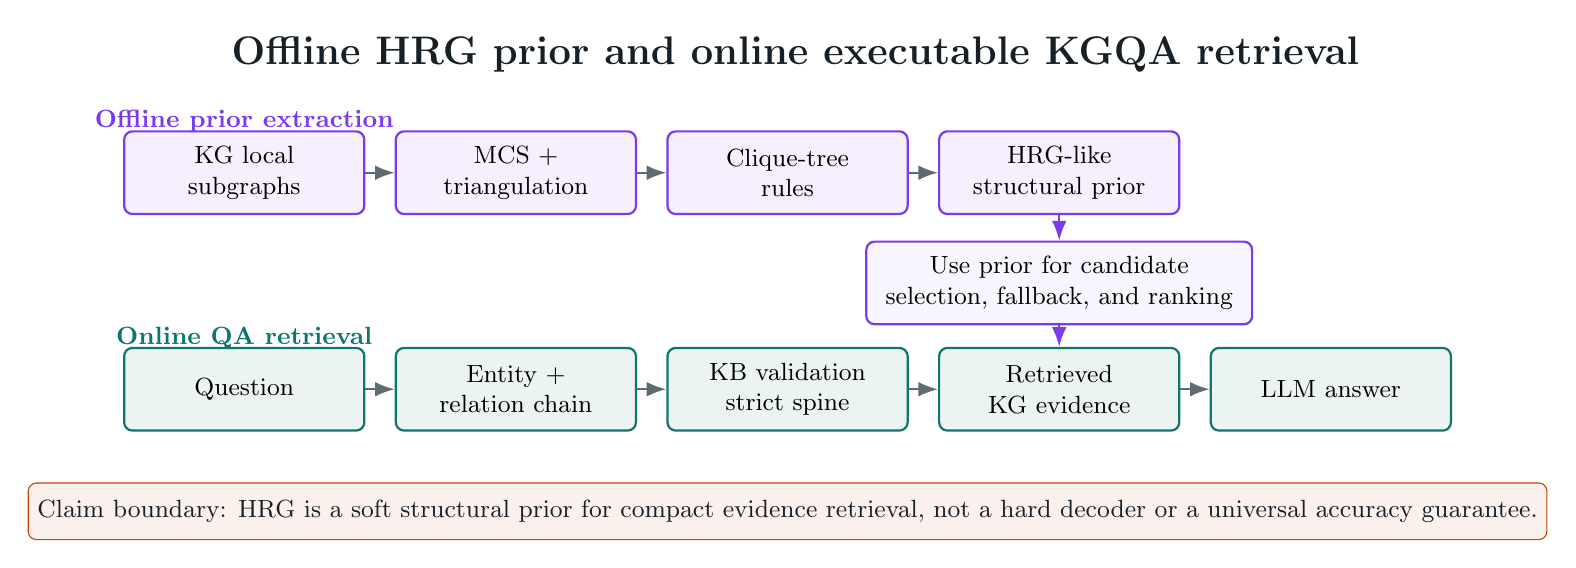
\begin{tikzpicture}[
  font=\sffamily,
  box/.style={rounded corners=3pt, draw=line, thick, fill=panel, minimum width=3.05cm, minimum height=1.05cm, align=center, font=\small},
  hbox/.style={box, draw=hrg, fill=hrg!8},
  obox/.style={box, draw=spine, fill=spine!8},
  pbox/.style={rounded corners=3pt, draw=hrg, thick, fill=hrg!5, minimum width=4.9cm, minimum height=1.05cm, align=center, font=\small},
  arrow/.style={-{Latex[length=2.5mm]}, thick, draw=muted},
]
\node[font=\bfseries\Large, text=ink] at (7.0,4.95) {Offline HRG prior and online executable KGQA retrieval};
\node[font=\bfseries\small, text=hrg] at (0,4.10) {Offline prior extraction};
\node[font=\bfseries\small, text=spine] at (0,1.35) {Online QA retrieval};

\node[hbox] (kg) at (0,3.45) {KG local\\subgraphs};
\node[hbox] (mcs) at (3.45,3.45) {MCS +\\triangulation};
\node[hbox] (clique) at (6.90,3.45) {Clique-tree\\rules};
\node[hbox] (grammar) at (10.35,3.45) {HRG-like\\structural prior};
\draw[arrow] (kg) -- (mcs);
\draw[arrow] (mcs) -- (clique);
\draw[arrow] (clique) -- (grammar);

\node[pbox] (prioruse) at (10.35,2.05) {Use prior for candidate\\selection, fallback, and ranking};
\draw[arrow, draw=hrg] (grammar.south) -- (prioruse.north);

\node[obox] (q) at (0,0.70) {Question};
\node[obox] (parse) at (3.45,0.70) {Entity +\\relation chain};
\node[obox] (valid) at (6.90,0.70) {KB validation\\strict spine};
\node[obox] (evid) at (10.35,0.70) {Retrieved\\KG evidence};
\node[obox] (ans) at (13.80,0.70) {LLM answer};
\draw[arrow] (q) -- (parse);
\draw[arrow] (parse) -- (valid);
\draw[arrow] (valid) -- (evid);
\draw[arrow] (evid) -- (ans);
\draw[arrow, draw=hrg] (prioruse.south) -- (evid.north);

\node[draw=warn, fill=warn!8, rounded corners=3pt, align=center, text=ink, minimum width=14.6cm, minimum height=0.72cm, font=\small] at (6.90,-0.85)
{Claim boundary: HRG is a soft structural prior for compact evidence retrieval, not a hard decoder or a universal accuracy guarantee.};
\end{tikzpicture}

\end{document}
